\chapter{Grundlagen}
\label{chap:grundlagen}

Wie bereits in der Einleitung erwähnt, sind Kameras ein wichtiger Sensor in der Robotik, indem sie dem Roboter helfen, die Umgebung wahrzunehmen. Abhängig von dem Einsatzgebiet, ist ein genaues Abbild der Umgebung außerordentlich wichtig für die Erfüllung der Aufgabe. Dies ist der Fall, wenn zum Beispiel der Roboter über das Kamerabild einen Gegenstand lokalisieren muss, um ihn anschließend zu greifen, oder er muss in dem Kamerabild Hindernisse erkennen, um einen Weg zum Ziel zu planen.

Der relativ günstige Preis von Lochkameras gegenüber anderen bildgebenden Sensoren hat dazu beigetragen, dass Kameras ein viel genutzter Sensor sind. Da sich aber gezeigt hat, dass die Toleranzen bei der Produktion und der Aufbau der Kameras an sich zu Verzerrungen im Bild führen, wurden Modelle entwickelt, um diese Verzerrungen herauszurechnen und das Bild zu korrigieren. Ein häufig genutztes Modell wird im folgenden beschrieben.

\section{Kameramodell} % (fold)
\label{sec:kameramodell}
In \cite{Zhang} wird ein gängiges Kameramodell beschrieben, welches nun kurz erklärt wird.

Die Beziehung zwischen einem Punkt $(u, v)$ in einem zweidimensionalen Bild und einem Punkt $(x, y, z)$ in der dreidimensionalen Welt wird durch \autoref{projection} beschrieben:

\begin{equation}
\begin{bmatrix}
 	u \\
 	v \\
 	1
\end{bmatrix} = K 
\begin{bmatrix}
   	R & T
\end{bmatrix} 
\begin{bmatrix}
   	x \\
   	y \\
   	z \\
   	1
\end{bmatrix} \label{projection}
\end{equation}

mit 

\begin{equation}
  K = 
  \begin{bmatrix}
  	f_x & 0 & c_x \\
  	0 & f_y & c_y \\
  	0 & 0 & 0
  \end{bmatrix}
\end{equation}

$K$ enthält die intrinsischen Parameter der Kamera, die auf Grund der Fertigungstoleranzen für jede Kamera unterschiedlich sind. $f$ definiert die Brennweite der Kamera. Da die Pixel nicht immer quadratisch sind, wird dieser Wert für die x und y-Achse angegeben. $c_x$ und $c_y$ beschreiben das optische Zentrum des Bildes, welches ebenfalls nicht immer genau im Mittelpunktes des Bildes liegt.

$R$ und $T$ definieren die extrinsischen Parameter. $R$ ist eine Rotationsmatrix, die die Rotation zwischen dem Kamera- und Weltkoordinatensystem beschreibt, $T$ ist ein Vektor, der die Transformation zwischen Kamera- und Weltkoordinatensystem beschreibt.

\section{Verzeichnung} % (fold)
\label{sec:verzeichnung}
Mit dem Kameramodell kann nun eine Beziehung zwischen einem Punkt im Bild und dem Punkt in der Welt hergestellt werden. Kameras bilden das Bild jedoch nicht immer korrekt ab. Häufig sieht man in Bildern den Effekt, dass gerade Linien in der Welt, wie z.B. Häuserkanten, nicht gerade im Bild aufgenommen werden, sondern das diese gebogen werden. Diesen Effekt nennt man Verzeichnung.

Man kann zwischen zwei verschiedenen Arten der Verzeichnung sprechen. Die Verzeichnung, die gerade Linien gekrümmt darstellt, heißt radiale Verzeichnung. Um diese Verzeichnung herauszurechnen, werden die drei Faktoren $k_1, k_2, k_3$ benötigt. Sind diese gegeben, lässt sich die Verzeichnung korrigieren. $r$ ist der Abstand vom Bildmittelpunkt zum Punkt, der korrigiert werden soll. $x', y'$ sind die falsch abgebildeten Punkte, $x,y$ sind die korrigierten Punkte.

\begin{equation}
	x = x'(1 + k_1 r^2 + k_2 r^4 + k_3 r^6)
\end{equation}
\begin{equation}
	y = y'(1 + k_1 r^2 + k_2 r^4 + k_3 r^6)
\end{equation}

Zusätzlich zu der radialen Verzeichnung gibt es tangentiale Verzeichnung. Diese tritt auf, wenn die Kameralinse nicht parallel zum Sensor eingebaut ist. Diese Verzeichnung führt dazu, dass Linien, die im idealen Bild parallel verlaufen, nun einen gemeinsamen Fluchtpunkt besitzen. Um diese Verzeichnung zu korrigieren, werden die Faktoren $p_1, p_2$ benötigt.

\begin{equation}
	x = x' + (2 p_1 xy + p_2 (r^2 + 2 x^2))
\end{equation}
\begin{equation}
	y = y' + (p_1(r^2 + 2 y^2) + 2p_2 xy)
\end{equation}

\section{Kalibrierung} % (fold)
\label{sec:kalibrierung}
Der Kalibrierungsvorgang dient dazu, die intrinsischen und gegebenenfalls extrinsischen Parameter, sowie die Verzeichnungsparameter zu berechnen. Dies erfolgt in mehreren Schritten.

\subsection{Kalibrierungsmuster} % (fold)
\label{sub:kalibrierungsmuster}
Man braucht ein Kalibrierungsmuster, von dem im nächsten Schritt einige Aufnahmen gemacht werden. Es gibt verschiedene Kalibrierungsmuster, die benutzt werden können. Eine grundlegende gemeinsame Eigenschaft aller Kalibrierungsmuster ist, dass das Muster aus geometrischen Formen besteht, die gut von Bilderkennungsalgorithmen gefunden werden können. Häufig wird dazu ein Schachbrettmuster benutzt, siehe \autoref{img:chess5x7x0.03}. In diesem Muster haben die Rechtecke eine Kantenlänge von exakt 3cm. Inge samt sind 6 x 8 Rechtecke in dem Muster vorhanden. Der Kalibrierungsalgorithmus sucht nach den Kanten der Quadrate. Der Schnittpunkt von zwei Kanten, also eine Ecke des Quadrats, bildet den Kalibrierungspunkt. Dadurch enthält ein Bild mit diesem Kalibrierungsmuster 5 x 7, also 35, Kalibrierungspunkte.

\begin{figure}[!hbt]
	\centering
	\vspace{1ex}
	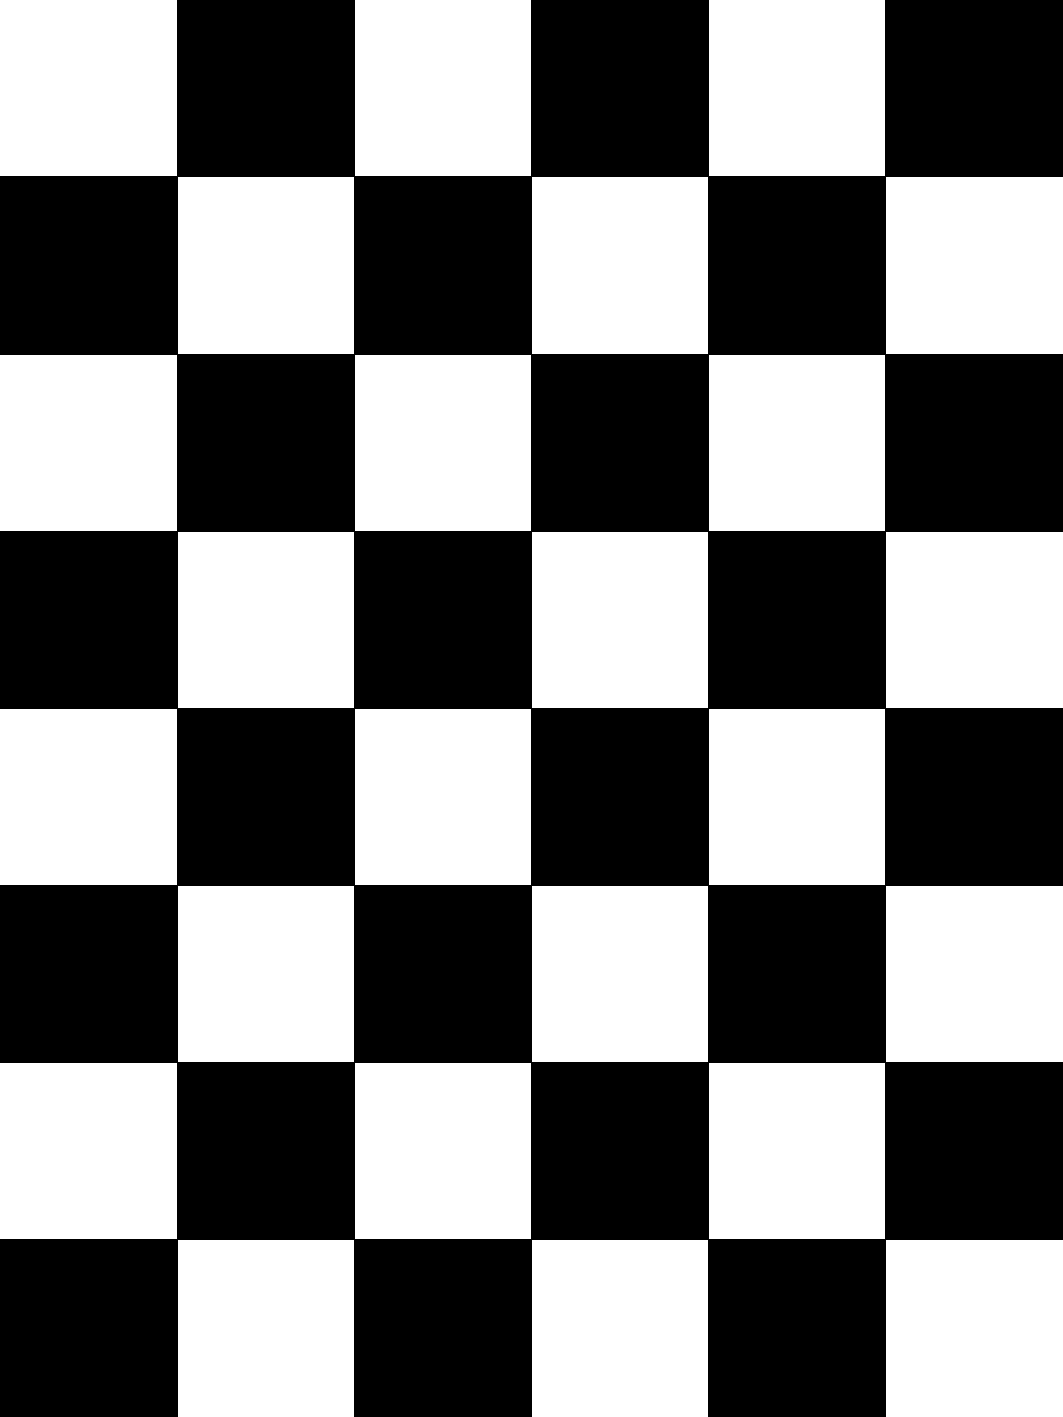
\includegraphics[scale=0.3, angle=90]{../images/chess5x7x3}
	\caption[Schachbrettmuster als Kalibrierungsmuster]{\label{img:chess5x7x0.03} Schachbrettmuster als Kalibrierungsmuster}
	\vspace{1ex}
\end{figure}

Ein anderes Kalibrierungsmuster besteht aus Kreisen, die regelmäßig versetzt zueinander positioniert sind, siehe \autoref{img:caltab_hex_10x11}. In diesem Muster sind die Mittelpunkte der Kreise die Kalibrierungspunkte. In diesem Muster sind 10 x 11 Kreise eingezeichnet, sodass deutlich mehr Informationen für die Kalibrierung in einer Aufnahme vorhanden sind. 

\begin{figure}[!hbt]
\centering
	\vspace{1ex}
	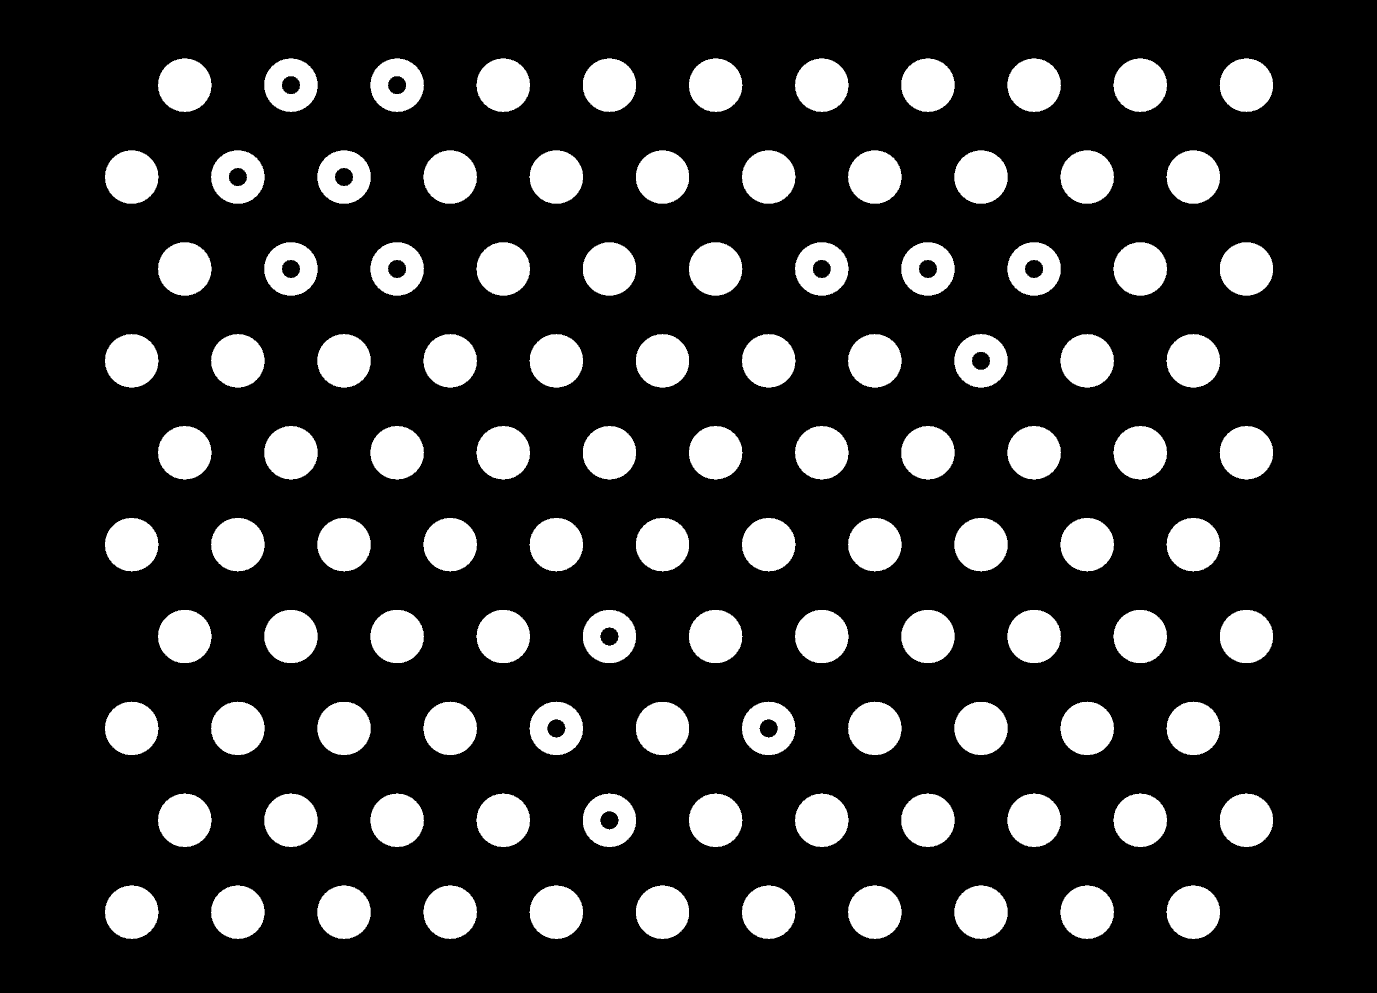
\includegraphics[scale=0.2]{../images/caltab_hex_10x11}
	\caption[Punkte als Kalibrierungsmuster]{\label{img:caltab_hex_10x11} Punkte als Kalibrierungsmuster}
	\vspace{1ex}
\end{figure}

Das Muster ist außerdem speziell für HALCON entwickelt. Während die Kreismuster von OpenCV im ganzen Bild den gleichen Punkt benutzen, sind in diesem Muster einige Punkte zusätzlich markiert. Dadurch kann HALCON auch dann noch Kalibrierungsinformationen aus einer Aufnahme errechnen, wenn das Kalibrierungsmuster nur teilweise zu sehen ist. Bei dem Schachbrettmuster oder dem Punktmuster von OpenCV muss hingegen immer das ganze Muster erkennbar sein.

Unabhängig davon, welches Muster man einsetzt, muss immer die Größe und Form der ausgedruckten Muster exakt den erwarteten Daten entsprechen. Da manche Drucker versuchen, die Dokumente auf DinA4-Größe anzupassen, muss man für jedes ausgedruckte Muster die Größe und Abstände der geometrischen Objekte überprüfen. Hat das ausgedruckte Muster die korrekte Größe, muss dieses auf eine möglichst ebene Oberfläche geklebt werden. Ein gekrümmtes Muster in einer Aufnahme, die zur Kalibrierung benutzt wird, kann die Ergebnisse verfälschen. 

\subsection{Bildaufnahme} % (fold)
\label{sub:bildaufnahme}
Damit der Kalibrierungsalgorithmus die Parameter berechnen kann, muss er aus mehreren Bildern die Kalibrierungspunkte extrahieren. Dabei wird an die Bilder, die zur Kalibrierung benutzt werden, mehrere Anforderungen gestellt. 

Wie bei anderen Fotos auch ist es wichtig, dass das Motiv, also das Kalibrierungsmuster, scharf dargestellt wird und gut belichtet ist. Dabei ist es hilfreich, wenn Kamera und Kalibrierungsmuster auf Stativen befestigt sind. 

Das Kalibrierungsmuster sollte außerdem in verschiedenen Distanzen aufgenommen werden. Andernfalls kann es passieren, dass die berechneten Parameter nur auf den Abstand passen, den das Kalibrierungsmuster zur Kamera während der Aufnahmen hatte. Möchte man nun mit diesen Parametern die Kamera benutzen und Objekte mit einem anderen Abstand beobachten, können die Parameter das Bild nun verschlechtern und die Bildinformationen passen nicht mehr zur Realität.

Nicht nur die Entfernung zur Kamera ist wichtig sondern auch die Orientierung des Kalibrierungsmusters. Indem man das Kalibrierungsmuster an jeder Position nach oben und unten sowie nach rechts und links neigt, verbessert man die Qualität der Kalibrierung.

Zuletzt sollte das Kalibrierungsmuster über alle einzelnen Bilder verteilt den ganzen Bildausschnitt füllen. Würden beispielsweise alle Bilder das Kalibrierungsmuster nur in der Bildmitte zeigen, könnten die Parameter so gewählt werden, dass die Bildmitte zwar sehr gut kalibriert ist, aber das Bild an den Bildrändern stark verzeichnet ist. 

\subsection{Berechnung der Parameter} % (fold)
\label{sub:berechnung_der_parameter}
Wurden genügend Bilder aufgenommen, die den Anforderungen entsprechen, können die Parameter berechnet werden. Dazu ist eine initiale Konfiguration der intrinsischen Parameter nötig. Die dafür notwendigen Informationen kann man den Spezifikationen der Kamera oder des Sensors entnehmen. Die Brennweite $f$ wird in der Regel vom Hersteller angegeben. Für das optische Zentrum $c_x$ und $c_y$ kann man die Bildmitte, also die halbe Auflösung des Bildes, annehmen.

Anschließend werden in jedem aufgenommenen Bild die Kalibrierungspunkte aus dem Bild extrahiert und abgespeichert. Als nächstes werden dann mit diesen Informationen die Gleichungssysteme gelöst, die die gesuchten Parameter enthalten. Zusätzlich zu den Parametern berechnen die Algorithmen den durchschnittlichen Fehler in Pixeln. Dieser sollte möglichst klein, am Besten unter 1 sein. Wird das Kalibrierungsmuster nicht in verschiedenen Orientierungen aufgenommen oder es ist nicht im ganzen Bildausschnitt zu sehen, kann dies den Fehler vergrößern.

Es gibt mehrere Frameworks, die man zum Kalibrieren benutzen kann. OpenCV ist eine freie Bibliothek zur Bildverarbeitung und maschinellen Sehen. Es wird kein fertiges Programm angeboten, mit dem der Vorgang direkt gestartet werden kann. Stattdessen existieren Bibliotheken in C++ und Python, in denen der Benutzer Funktionen findet, mit denen er sein eigenes Programm schreiben kann, um eine Kamera zu kalibrieren. Für Benutzer, die sich mit der Materie nicht so gut auskennen, ist dies eine hohe Hürde, Profis können damit aber das Programm auf die eigenen Bedürfnisse anpassen.

Ein anderes Framework ist HALCON. HALCON wird kommerziell vermarktet und ist nicht frei verfügbar. Es werden wie bei OpenCV Bibliotheken für verschiedene Programmiersprachen angeboten, mit denen Benutzer ihre eigenen Programme schreiben können. Zusätzlich existiert mit HDevelop eine integrierte Entwicklungsumgebung. In HDevelop wird eine eigene Programmiersprache benutzt, die weniger tief und detailliert als anderen Sprachen ist, aber dafür für unerfahrene Benutzer deutlich sprechender und intuitiver zu benutzen ist. Außerdem ist ein Kalibrierungsassistent enthalten, der die aufgenommen Bilder vor der Berechnung der Parameter anhand ihrer Bildschärfe, Belichtung und weiterer Eigenschaften bewertet.